\documentclass[12pt,a4paper,oneside,openright]{article}

\usepackage[utf8]{inputenc}
\usepackage[italian]{babel}
\usepackage[T1]{fontenc}
\usepackage{latexsym}
\usepackage{graphicx}
\usepackage{epsfig}
\usepackage{amsmath,amssymb,amsthm}
\usepackage[none]{hyphenat} 
\usepackage{float} % parametro H in figur : posizionamento esattamente li
\usepackage{verbatim}
\usepackage{booktabs}
\usepackage{enumerate} %lettere o altro negli indici
\usepackage{algorithmic} %float con un algoritmo
\usepackage[boxed]{algorithm}
\usepackage{subfig}    % + figure in un float figure

%con la classe book+openright lascio una pagina bianca a fine capitolo e dopo il titolo se necessario, con empty page queste pagine non sono numerate e non hanno stile
%%\usepackage{emptypage}



\usepackage{fancyhdr}
\setcounter{tocdepth}{3}

\makeatletter

% 1 freccia andata ritorno per scriverci sopra
\newcommand{\xleftrightarrow}[2][]{%
  \ext@arrow3399{\longleftrightarrowfill@}{#1}{#2}}
\newcommand{\longleftrightarrowfill@}{%
  \arrowfill@\leftarrow\relbar\rightarrow}

% 2 frecce andata ritorno per scriverci sopra
\def\rightharpoonupfill@{%
  \arrowfill@\relbar\relbar\rightharpoonup}
\def\leftharpoondownfill@{%
  \arrowfill@\leftharpoondown\relbar\relbar}


\newcommand{\xrightleftharpoons}[2][]{\mathrel{%
\raise.22ex\hbox{%
$\ext@arrow 3095\rightharpoonupfill@{\phantom{#1}}{#2}$}%
\setbox0=\hbox{%
$\ext@arrow 0359\leftharpoondownfill@{#1}{\phantom{#2}}$}%
\kern-\wd0 \lower.22ex\box0}%
}

\renewcommand{\algorithmicrequire}{\textbf{Input:}}
\renewcommand{\algorithmicensure}{\textbf{Output:}}

\makeatother 
\frenchspacing
%\pagestyle{headings} % {headings,plain ,empty}
\linespread{1.3}
\DeclareGraphicsRule{.eps,.ps,.png}{bmp}{.bb}{} % formati utilizzabili con ordine di preferenza 
                                                % cosi non devo indicare le estensioni
\newcommand{\HRule}{\rule{\linewidth}{0.5mm}}


%\author{\emph{Marco Bettiol}\quad{} 586580\\\emph{Antonio Quercia}\quad{}  588537}

%per impaginare con giustifica sx-dx
  \tolerance 1414
  \hbadness 1414
  \emergencystretch 1.5em
  \hfuzz 0.3pt
  \widowpenalty=10000
  \vfuzz \hfuzz
  \raggedbottom

\title{}
\begin{document}
% !TEX root = tesi.tex
\begin{titlepage}

		\thispagestyle{empty}
    \begin{figure}
    \centering
      \subfloat{
\includegraphics[scale=1]{immagini/logo_unipd_black}}\quad     \subfloat{
\includegraphics[scale=1.3]{immagini/DEIlogoFULL}}
    \end{figure}
    
    \vskip 3cm{
    \begin{center}\sc
        UNIVERSITY OF PADUA\\
        DEPARTMENT OF INFORMATION ENGINEERING\\
        MASTER DEGREE IN COMPUTER ENGINEERING\end{center}
		}
		
		\vskip1.2cm\begin{center}
      \rm\large\uppercase\expandafter{A.A. 2009/2010\\}
 \end{center}
    	
    \vskip 2.5cm\begin{center}
    \HRule \\[0.4cm]\LARGE\expandafter{BATCH SIZE ESTIMATE}
    \HRule \\[0.4cm]
    \end{center}
    
    \begin{flushright}\vskip4.0cm 
    \begin{tabular}{rl}
            \rm\large \uppercase{Supervisor:} &\emph{Prof. Andrea Zanella}\\
	   \rm\large \uppercase{Student:} &\emph{Marco Bettiol} \\
		\end{tabular}
     \end{flushright}
    \vfill
          \begin{center}
                  \vskip1.0cm 
                  Last Update: \today  \hspace{1mm } \currenttime
           \end{center}
    
\end{titlepage}

\newpage
%%pagina vuota
%\clearpage\null\thispagestyle{empty}\clearpage

%\setcounter{page}{1}

%\tableofcontents

\section*{Introduzione}
Un vettore $x$ di lunghezza N può essere visto come una sequenza $x_0,...,x_{N-1}$ di N numeri complessi. Si definisce $X$ \emph{trasformata discreta di Fourier (DFT, discrete Fourier transform)}  di $x$ la sequenza $X_0,...,X_{N-1}$ espressa dalla seguente relazione:
\begin{equation*}
\label{eq:def-dft}
X_k=\sum_{n=0}^{N-1}x_ne^{-\jmath\frac{2\pi}{N}kn} \quad k=0,...,N-1
\end{equation*}
La \emph{FFT} o \emph{trasformata veloce di Fourier} individua una famiglia di algoritmi in grado di calcolare la DFT in tempo $O(N \log N)$ al posto dell'usuale $O(N^{2})$ ottenibile banalmente attraverso la definizione.\\
Molti di questi algoritmi, oltre che ad essere computazionalmente efficienti, si prestano bene anche ad un'implementazione parallela.\\
In questo lavoro è stata realizzata un'implementazione del noto algoritmo di Cooley-Tukey.
\section{Algoritmo}
L'algoritmo di Cooley-Tukey prevede di calcolare la DFT del vettore $x$ attraverso il calcolo separato delle DFT delle sottosequenze di indice pari e dispari della sequenza originaria e quindi la loro ricombinazione attraverso \emph{operazioni butterlfy} tra elementi in posizione analoga delle due sottosequenze per ottenere la trasformata della originale.\\
L'immagine seguente illustra quanto appena enunciato per una sequenza di lunghezza 8
\begin{figure}[H] 
  \centering
      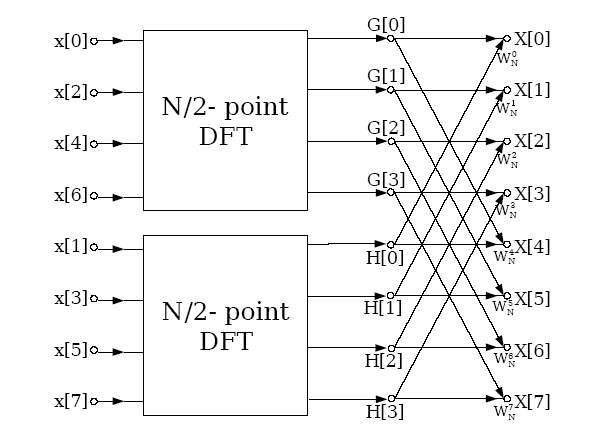
\includegraphics[width=\textwidth]{immagini/cooley-tukey}
  \caption{Ricombinazione in Cooley-Tukey per una sequenza di lunghezza 8}
\end{figure}
Questo rimescolamento dell'input iniziale, operato a ritroso fino al caso base di sequenze di lunghezza 2, permette di notare come l'algoritmo di CT sia costituito da una rete ascendente che ha come input il vettore originale rimescolato in ordine \emph{bitreversal}.
\begin{figure}[H] 
  \centering
      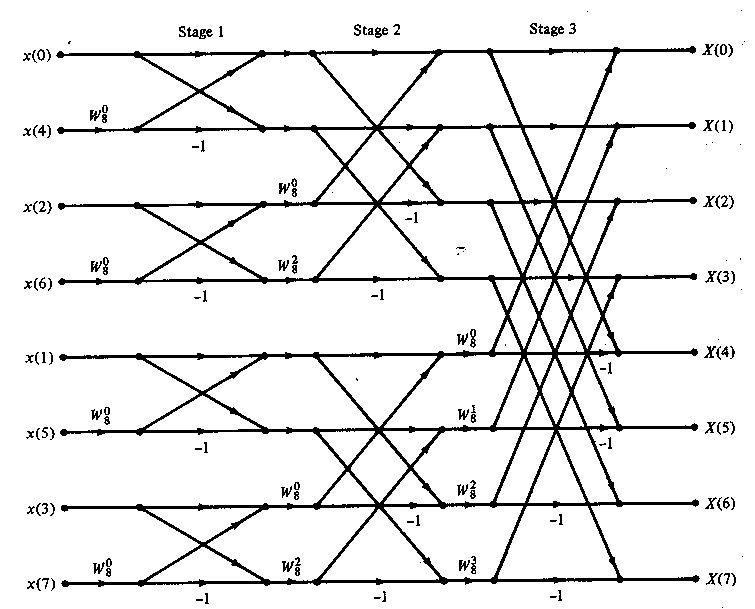
\includegraphics[width=\textwidth]{immagini/alg-asc}
  \caption{bitreversal di una sequenza di lughezza 8 e computazione su rete ascendente}
\end{figure}
Ora, considerando una sequenza di lunghezza N e avendo a disposizione P processori, è possibile dividere la sequenza iniziale in P blocchi da $\frac{N}{P}$ elementi. Il processore $i$-esimo sarà responsabile dell'$i$-esimo blocco. Notiamo come la computazione sia inizialmente priva di comunicazioni in quanto ogni processore dispone localmente dei dati da elaborare. Soltanto le ultime $\log_{2} P$ fasi richiedono infatti l'utilizzo di dati di responsabilità di un altro processore. In queste fasi che chiameremo ``esterne'' (analogamente consideriamo ``interne'' le fasi precedenti), il processore $x$, utilizzando la notazione vista a lezione, comunicherà prima con $C_{0}x$, quindi con $C_{1}x$,...
In generale, nella $j$-esima fase esterna, si avrà lo scambio dei rispettivi blocchi di responsabilità tra
$$x  \longleftrightarrow  C_{j}x \quad \textrm{per} \quad j=0,...,\log_{2} P-1 $$

\section{Implementazione}
Per prima cosa è stata sviluppata un'implementazione sequenziale iterativa dell'algoritmo di CT cercando di seguire i suggerimenti visti a lezione per quanto riguarda l'ottimizzazione del codice. I cicli (3) utilizzati per la computazione sono stati modificati in modo da essere decrescenti (es: da N-1 a 0) e ordinati in modo da elaborare il vettore dei dati in maniera contigua (posizione i, i+1, e così via) al fine di ridurre gli accessi ed utilizzare nel modo migliore RAM e soprattutto cache.\\
Particolare attenzione è stata inoltre riposta nella gestione dei \emph{twiddle factors}.\\
Per elaborare una sequenza di lunghezza N è necessario calcolare $\frac{N}{2}$ \emph{twiddle factors} ($ \omega_{N}^{0},...,\omega_{N}^{\frac{N}{2}-1}$). Tuttavia soltanto nell'ultima fase vengono utilizzati tutti i \emph{twiddle factors} mentre nelle fasi precedenti si utilizzano solo alcuni di questi (ottenibili come un sottocampionamento del vettore appena calcolato). Ad esempio nella prima fase si utilizza, banalmente, $ \omega_{N}^{0}=1$, nella seconda $ \omega_{N}^{0}$ e $\omega_{N}^{\frac{N}{4}}=-j$, nella terza $ \omega_{N}^{0}$, $\omega_{N}^{\frac{N}{8}}$, $\omega_{N}^{\frac{N}{4}}$, $\omega_{N}^{\frac{3N}{8}}$ e così via.\\
Pertanto sottocampionando progressivamente il vettore \emph{twiddle factors} mantenendo solo gli elementi in posizione dispari si è prodotto un vettore di lunghezza 2N-1 che ha in posizioni contigue i \emph{twiddle factors} opportuni che saranno impiegati in ciascun stadio. Con uno ``spreco'' di $\frac{N}{2}$ di RAM ulteriormente occupata è stato pertanto ottimizzato l'accesso in RAM/cache ai fattori di ricombinazione. Questo ha fornito un ulteriore boost prestazionale molto evidente.\\
L'implementazione sequenziale così ottenuta è stata quindi utilizzata come base di partenza per:
\begin{enumerate}
\item un algoritmo ascendente con chiamate bloccanti
\item un algoritmo ascendente con chiamate non-bloccanti
\end{enumerate}
\subsection{Sceletro generale dell'algoritmo}

Il processore con rank 0 è eletto come coordinatore del gruppo di processori e si occupa della gestione, distribuzione e raccolta dei dati elaborati.

Le fasi principali che possiamo individuare dall'algoritmo sono:
\begin{enumerate}
\item $P_{0}$ legge l'input da file o lo genera se richiesto
\item $P_{0}$ dispone l'input in bit-reversal
\item Ogni processore calcola localmente i \emph{twiddle factors} e li memorizza in un vettore
\item $P_{0}$ distribuisce a ciascun processore la porzione di input di cui è responsabile attraverso una chiamata MPI\_Scatter
\item Calcolo della FFT parallela prima nelle dimensioni interne e poi in quelle esterne
\item $P_{0}$ raccoglie i risultati attraverso un MPI\_Gather
\item $P_{0}$ scrive l'eventuale output
\end{enumerate}
 
\subsubsection{Algoritmo ascendente bloccante}
Per l'implementazione della modalità bloccante, poichè ogni processore manda dati e li riceve dallo stesso ``collega'' si è utilizzata la primitiva
\begin{verbatim}
MPI_Sendrecv(sendbuf, sendcount, sendtype, dest, sendtag, recvbuf, 
               recvcount, recvtype, source, recvtag, comm, status)
\end{verbatim} 
che prevede lo scambio mutuo di dati tra due processori.  
\subsubsection{Algoritmo ascendente non-bloccante}
Come già detto ogni processore gestisce $\frac{N}{P}$ elementi memorizzati in un vettore.\\
Denominiamo con A e B rispettivamente la prima e la seconda metà del vettore (A e B contengono quindi $\frac{N}{2P}$ elementi ciascuno). Indichiamo inoltre con A' e B' i dati provenienti dal processore ``collega''.
Per ogni stadio (completo) in cui è necessaria la comunicazione con altri processori questa avviene nel seguente modo:
\begin{enumerate}
\item Attesa per il completamento della ricezione di B' e l'invio di B
\item Aggiornamento di B
\item Invio di B e ricezione di B' 
\item Attesa per il completamento della ricezione di A' e l'invio di A
\item Aggiornamento di A
\item Invio di A e ricezione di A'  
\end{enumerate}
In questo caso le primitive utilizzate sono quelle non bloccanti, non bufferizzate
\begin{center}
\begin{verbatim}
                MPI_Isend, MPI_Irecv, MPI_Wait 
\end{verbatim} 
\end{center}
La scelta di suddividere il vettore in due metà e comunicarne prima l'una e poi l'altra è nata dall'idea di
\begin{enumerate}
\item limitare l'impatto del costo della gestione della comunicazione. Infatti tanto più sovrapposte sono calcolo e comunicazione (pacchetti scambiati piccoli) tanto più sforzo è richiesto alla macchina per la gestione dei buffer della comunicazione
\item cercare di limitare il ritardo dovuto alla comunicazione a quello dell'invio di $\frac{N}{2P}$ elementi + delay iniziale. 
\end{enumerate}

\subsection{Modalità d'uso}

Il software sviluppato funziona per
\begin{itemize}
\item $N=2^{n}$; lunghezza della sequenza da elaborare
\item $P=2^{p}$; numero di processori impiegati
\item $P<N$; quindi risulta $\frac{N}{P}\geq 2$ in modo da avere come caso base sempre operazioni tra due elementi.
\end{itemize}

\noindent Il programma prevede 2 distinte modalità di esecuzione.\\
La prima è utile per la valutazione delle performance dell'algoritmo, la seconda per l'effettivo impiego.
Consideriamo $n=\log_{2}N$
\begin{description}
\item[ Test su sequenza nota ] Il nodo $P_{0}$ genera un'input di lunghezza $2^{n}$  e quindi procede con il calcolo parallelo della sua FFT. \\ La sintassi è:
\begin{verbatim}
      ./fft-asc-* test n
\end{verbatim}
\item[ Elaborazione dell'input fornito]  $P_{0}$ legge da file l'input che dopo l'elaborazione viene salvato in un file di output
\begin{verbatim}
      ./fft-asc-* read n file_input file_output
\end{verbatim}
dove *$\in$\{sp, cp\} per richiamare rispettivamente la versione bloccante o non bloccante.
\end{description}
\subsection{Formato dei file elaborati}
Il i file sono letti/scritti con \emph{fscanf}  / \emph{fprintf}. I file devono essere costituiti da una sequenza di coppie di numeri intervallati da spazi o return. Per ciascuna coppia il primo elemento viene interpretato come parte la reale mentre il secondo come parte immaginaria dell'effettivo valore da elaborare.\\
Ad esempio:\\
\begin{center}
\fbox{\parbox[c]{2cm}{\begin{center}0 0\\ 1 0\\  2 0\\ 3 0\end{center}}} $\longleftrightarrow$\fbox{\parbox[c]{2cm}{\begin{center}0 0 1\\ 0  2 0\\ 3 0\end{center}}} $\longleftrightarrow$ \fbox{\parbox[c]{2cm}{\begin{center}$0+j0$\\$ 1+j0$\\  $2+j0$\\ $3+j0$\end{center}}} 
\end{center}


\section{Prestazioni}




\subsubsection*{Breve confronto tra le due implementazioni sequenziali}
Notiamo come all'aumentare della taglia del problema l'ottimizzazione e la migliore gestione della cache aumentino considerevolmente le prestazioni.
\begin{figure}[H]
  \centering 
  \subfloat[1. Tempi di calcolo assoluti in secondi tra le due implementazioni]{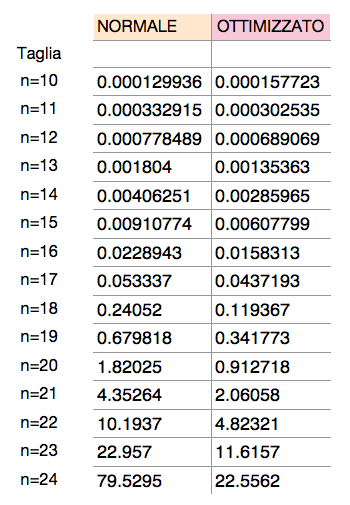
\includegraphics[width=0.40\textwidth]{immagini/confronto_sequenziale_tempi}}\quad   \subfloat[4. Guadagno dell'algoritmo ottimizzato]{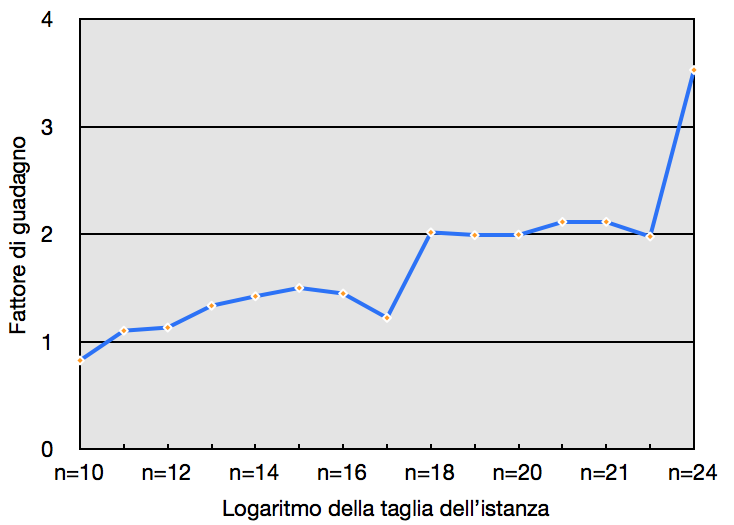
\includegraphics[width=0.55\textwidth]{immagini/guadagno_sequenziale}}   
\end{figure}

\subsection{Analisi Parallela}
L'algoritmo parallelo ``naive'' (basato sul codice non ottimizzato) e quello ottimizzato sono stati eseguiti un numero di volte tra 25 e 200 (in funzione della taglia dell'input) in modo da ricavare i tempi medi di esecuzione con un'affidabilità adeguata.

I test sono stati tutti eseguiti con la comunicazione attraverso memoria condivisa abilitata (\emph{MP\_SHARED\_MEMORY = yes}) e selezionando lo switch ad alte prestazioni per la comunicazione tra nodi (\emph{network.mpi    $=$  switch,shared,US})
\subsubsection{Test con carico massimo sui nodi}
Per prima cosa entrambi gli algoritmi sono stati lanciati con il parametro \emph{blocking = unlimited} nei file .job. In questa modalità vengono allocati per ogni nodo il maggior numero di processori possibile in modo da ridurre il più possibile il tempo dovuto alle comunicazioni tra processori di nodi diversi. \\

\begin{figure}[H] 
  \centering
       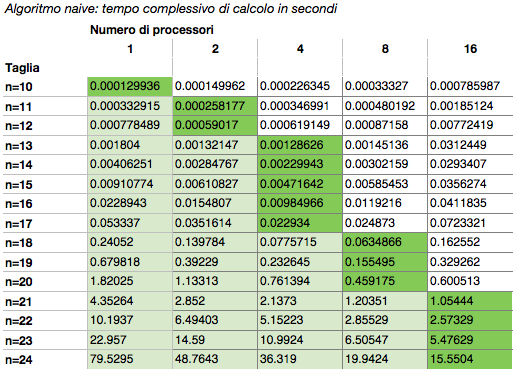
\includegraphics[ width=\textwidth]{immagini/algoritmo_normale_tempo_calcolo_senza_rete}
  \caption{In verde scuro il miglior tempo. In verde chiaro i tempi descrescenti}
\end{figure}
\begin{figure}[H] 
  \centering
      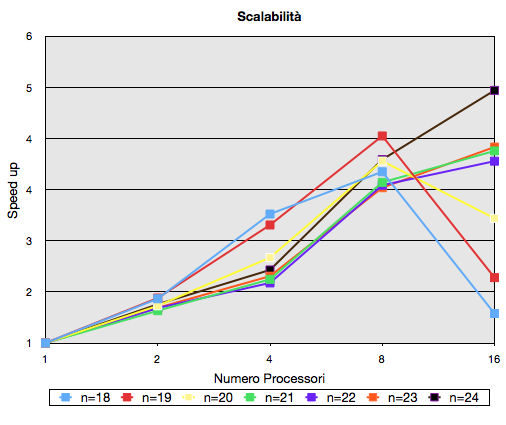
\includegraphics[ height=0.4\textheight]{immagini/scalabilita_normale_senza_rete}
	\caption{\textsf{Algoritmo naive} con \emph{blocking = unlimited}, scalabilità per taglie tra $2^{18}$-$2^{24}$}
\end{figure}
\begin{figure}[H] 
  \centering
      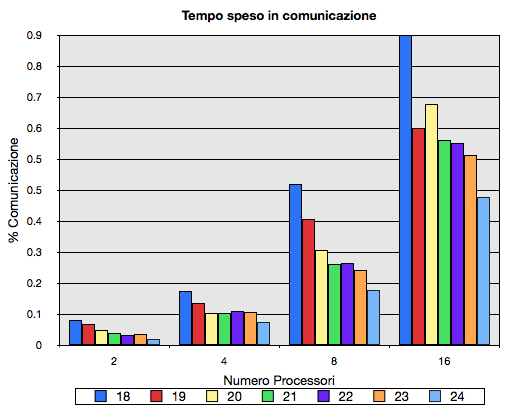
\includegraphics[height=0.4\textheight]{immagini/comunicazione_normale_senza_rete}
    \caption{\textsf{Algoritmo naive} con \emph{blocking = unlimited}, \% di tempo speso in comunicazione per taglie tra $2^{18}$-$2^{24}$}
\end{figure}

\begin{figure}[H] 
  \centering
       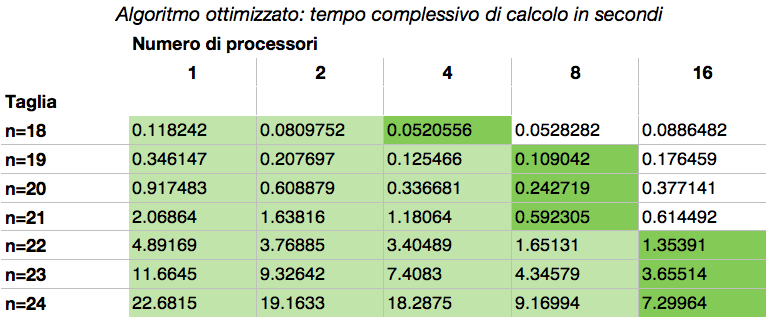
\includegraphics[ width=\textwidth]{immagini/algoritmo_ottimizzato_tempo_calcolo_senza_rete}
  \caption{In verde scuro il miglior tempo. In verde chiaro i tempi descrescenti}
\end{figure}
\begin{figure}[H] 
  \centering
      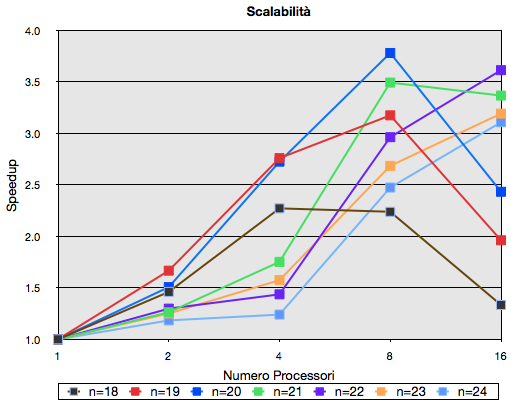
\includegraphics[height=0.4\textheight]{immagini/scalabilita_ottimizzata_senza_rete}
        \caption{\textsf{Algoritmo ottimizzato} con \emph{blocking = unlimited}, scalabilità per taglie tra $2^{18}$-$2^{24}$}
\end{figure}
\begin{figure}[H] 
  \centering
      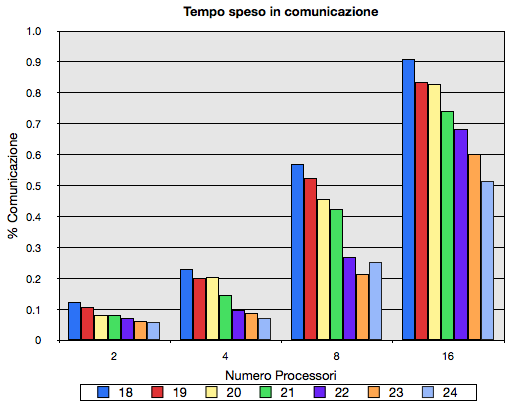
\includegraphics[height=0.4\textheight]{immagini/comunicazione_ottimizzata_senza_rete}
 	  \caption{\textsf{Algoritmo ottimizzato} con \emph{blocking = unlimited}, \% di tempo speso in comunicazione per taglie tra $2^{18}$-$2^{24}$}
\end{figure}

Dalle tempistiche assoulte emerge come per entrambe le versioni al crescere della taglia ci sia un continuo miglioramento fino al punto critico in cui il costo della comunicazione sovrasta quello effettivo di calcolo. Poichè l'algoritmo ottimizzato è più efficiente a livello sequenziale l'impatto della comunicazione lo penalizza maggiormente: questo è evidente dal fatto che sebbene i risultati assoluti siano sempre molto migliori, lo speedup parallelo è inferiore. Inoltre, per problemi di taglia modesta o piccola, si ha che il punto di trade-off in cui è controproducente utilizzare più processori è anticipato rispetto all'algoritmo naive. 

I grafici mostrano, inaspettatamente, che con pochi processori, sono proprio i problemi con taglia n=18, n=19 a trarre il maggior beneficio dall'utilizzo di 2 e 4 processori.

Osservando la tabella dei tempi di comunicazione della tabella seguente si osserva come nel passaggi da 2 a 4 processori il tempo, pur raddoppiando, rimanga contenuto e tuttavia il tempo complessivo impiegato dall'algoritmo migliora solo marginalmente : con un raddoppio di processori si ha un miglioramento solo lineare.

\begin{figure}[H] 
  \centering
      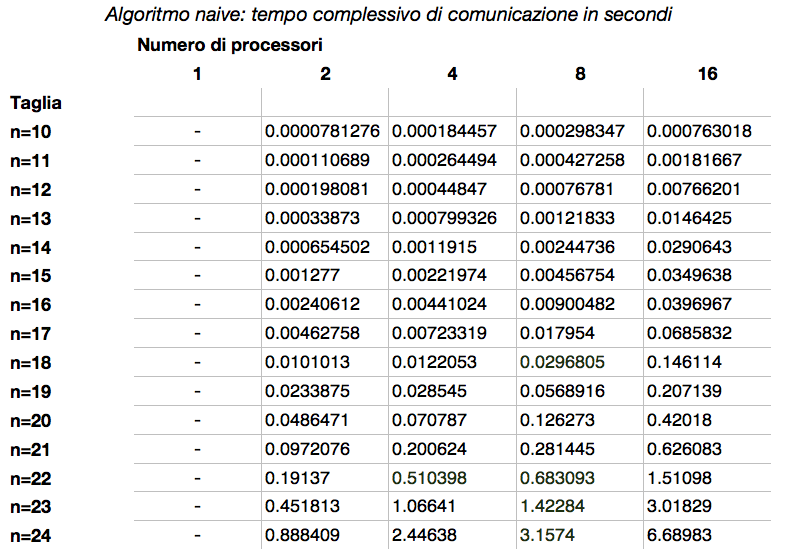
\includegraphics[width=\textwidth]{immagini/algoritmo_normale_tempo_comunicazione_senza_rete}
\end{figure}

Passando ad 8 processori si verifica però un miglioramento più che doppio rispetto al caso con 4. Questo ci fa supporre che ci sia qualche collo di bottiglia che deve essere considerato (vedremo in seguito).

Come ultime osservazioni notiamo come nell'algoritmo ottimizzato non sia ancora arrivato al limite di scalabilità con le taglie di problemi prese in esame: infatti lo speedup per 8 o 16 processori risulta inferiore al crescere della taglia (es:  per n=22,n=23,n=24) ma taglie maggiori hanno un trend di miglioramento più promettente. Sebbene il costo di comunicazione sia proporzionalmente maggiore per taglie inferiori (e questo dovrebbe pertanto penalizzarle) si ha che, raddoppiando il numero di processori dimezza il rapporto $\frac{N}{P}$, il guadagno a livello sequenziale è più che doppio (anche triplo in alcuni casi) e questo boost dovuto ad un utilizzo migliore della cache fornisce risultati significativi.

Possiamo dire, prima di passare all'analisi del caso seguente, che i grafici non rispecchiano minimamente quanto ci si aspetterebbe dalla teoria e sono assai dissimili dal caso ideale.

\subsubsection{Test con carico minimo sui nodi}

Questi test sono stati condotti con \emph{blocking = 1} per 2 e 4 processi. Avendo solo al più 6 nodi per 8 e 16 processi si è dovuto ripiegare su \emph{blocking = 2} nel primo caso e \emph{blocking = 4} equivalente ad \emph{unlimited} nel secondo (pertanto con 16 processi si ricade nel test precedente). 

\begin{figure}[H] 
  \centering
      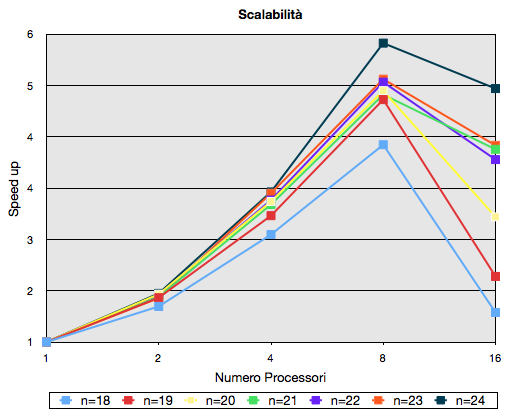
\includegraphics[ height=0.4\textheight]{immagini/scalabilita_normale_con_rete}
  \caption{\textsf{Algoritmo naive} con \emph{blocking = ``minimo''}, scalabilità per taglie tra $2^{18}$-$2^{24}$}
\end{figure}

\begin{figure}[H] 
  \centering
      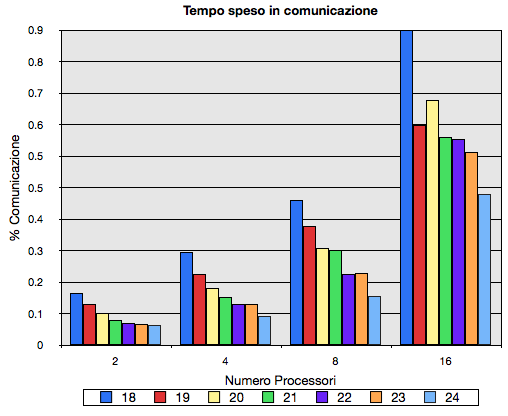
\includegraphics[height=0.4\textheight]{immagini/comunicazione_normale_con_rete}

    \caption{\textsf{Algoritmo naive} con \emph{blocking = ``minimo''}, \% di tempo speso in comunicazione per taglie tra $2^{18}$-$2^{24}$}
\end{figure}

\begin{figure}[H] 
  \centering
      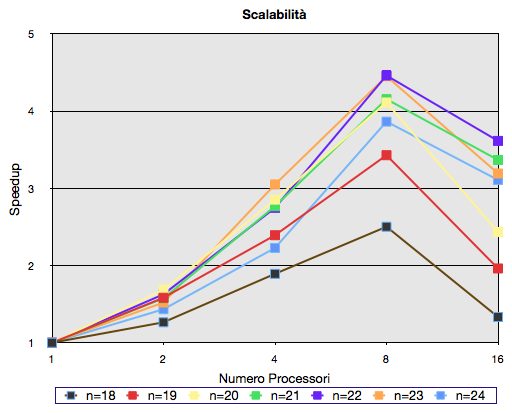
\includegraphics[ height=0.4\textheight]{immagini/scalabilita_ottimizzata_con_rete}
        \caption{\textsf{Algoritmo ottimizzato} con \emph{blocking = ``minimo''}, scalabilità per taglie tra $2^{18}$-$2^{24}$}
\end{figure}

\begin{figure}[H] 
  \centering
      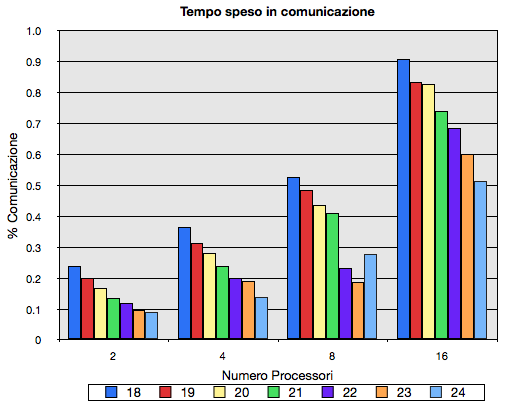
\includegraphics[height=0.4\textheight]{immagini/comunicazione_ottimizzata_con_rete}
  \caption{\textsf{Algoritmo ottimizzato} con \emph{blocking = ``minimo''}, \% di tempo speso in comunicazione per taglie tra $2^{18}$-$2^{24}$}
\end{figure}

Nei grafici ora l'effettto ``sella'' del passaggio da 4 a 8 processori è sparito. 

L'algoritmo naive ripercorre l'andamendo del grafico di scalabilità ideale in cui a taglie maggiori corrispondono speedup più elevati.
Notiamo come, sebbene il costo di comunicazione con 2 processori sia ora più elevato (circa il doppio) in quanto per la comunicazione viene ora sfruttata lo switch, le prestazioni fornite siano migliori rispetto a quelle ottenute in precedenza al variare di tutte le taglie/ numero di processori impegati.
Questo è possibile poichè ora, visto che non abbiamo più contesa tra i processori per l'accesso alla RAM (almeno con 2 e 4 processi), l'algoritmo sequenziale opera con piena efficienza.
Notiamo altresi osservando la tabella dei tempi sottostante come il tempo di comunicazione rimanga invariato al crescere del numero di processori impiegati da 2 a 8.
\begin{figure}[H] 
  \centering
      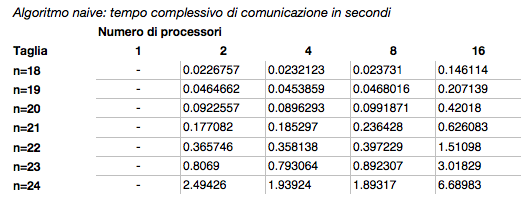
\includegraphics[width=\textwidth]{immagini/algoritmo_normale_tempo_comunicazione_con_rete}
\end{figure}

Ora entrambi gli algoritmi con soli 8 processori forniscono risultati migliori di quanto ottenuto nel test precedente.

Osservando la tabella dei tempi di calcolo totali (sotto) per l'algoritmo ottimizzato con \emph{blocking = ``minimo''} notiamo come il costo di comunicazione via rete, essendo molto elevato per le taglie di problema più piccole, renda l'esecuzione dell'algoritmo in questa configurazione controproducente per n=10,...,n=14 e sia poco scalabile per  n=15,...,17.
\begin{figure}[htp] 
  \centering
      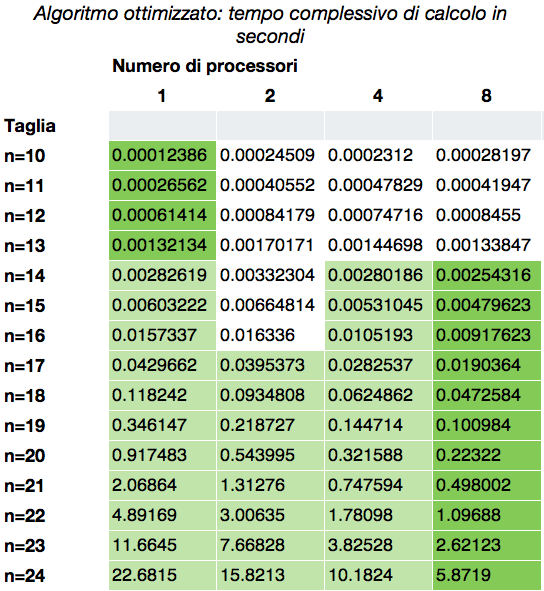
\includegraphics[width=0.7\textwidth, height=0.43\textheight]{immagini/algoritmo_ottimizzato_tempo_calcolo_con_rete}
\end{figure}
Il mantenersi stabile del costo di comunicazione fa si che vi siano dimensioni dell'istanza (n=14,n=15,n=16) per cui l'utilizzo di 2 processori è penalizzante mentre l'utilizzo di ben 8 risulta essere il caso più vantaggioso.

\subsubsection{Note su FFT Sequenziale e Cache}
Durante l'implementazione dell'algoritmo è emersa la critica dipendenza tra le prestazioni ottenute dall'algoritmo FFT-DIT2 rispetto alla dimensione della cache della macchina su cui viene lanciato.\\
L'algoritmo implementato infatti, per la natura stessa degli operatori \emph{butterfly}, risulta assolutamente non-cachefriendly.\\
L'accesso in memoria non è locale: ad ogni stadio dell'algoritmo un valore dell'input viene letto/sovrascritto una ed una sola volta. Quando l'accesso ai dati non è spazialmente localizzato e la struttura di computazione è rigida la classica modalità di mapping\\
\begin{center}
\emph{cache address} $=$ \emph{memory address} modulo \emph{cache\_size} 
\end{center}
perde di efficacia. Nel nostro caso si verifica quando la distanza tra i dati da elaborare (potenza di due) è vicina alla dimensione della cache (anch'essa potenza di due).\\
Proponiamo qui di seguito i grafici sullo Cache Miss e MFlops per illustrare la drammaticità del problema.\\
In entrambi i casi le performance diminuiscono drasticamente quando la taglia del problema supera $2^{15}=32768$ (che corrisponde a un vettore di \emph{twiddle factors} di esattamente 64KB: pari alla dimensione della cache L1 del processore) per mantenersi successivamente costanti fino a $2^{22}$ (vettore di 8MB pari alla cache L2).\\ La diminuzione praticamente lineare delle performance per $n=16$ visibile in Figura \ref{Miss} è conseguenza raddoppio del numero di \emph{twiddle factor} utilizzati ad ogni passo.\\
Le performance inferiori, a parità di stage, per le istanze di taglia maggiore sono probabilmente dovute allo swap in/out dei twiddle factor il cui address mapping entra in conflitto con quello dei valori nel vettore da elaborare.\\
Una volta oltrepassata la soglia critica il Loads per Miss si stabilizza sui $5,92$ più di $100$ volte peggiore rispetto agli stage in-cache. 
Analogamente per gli stage out-of-cache si hanno circa $81/60$ Mflops/s.

\begin{figure}[h!]
  \centering
      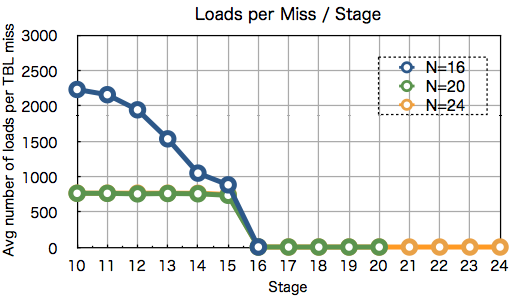
\includegraphics[width=0.8\textwidth]{immagini/Miss}
  \caption{Caricamento di dati utili nei registri / accessi in ram. Maggiore è migliore}
\label{Miss}
\end{figure}

\begin{figure}[h!] 
  \centering
      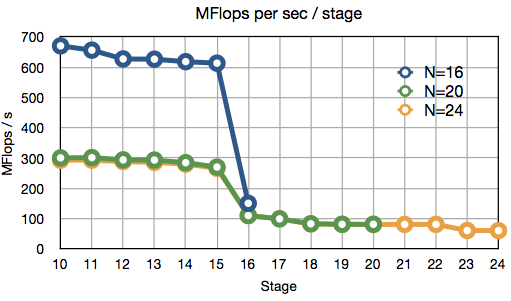
\includegraphics[width=0.8\textwidth]{immagini/Mflops}
  \caption{Potenza di calcolo sfruttata. Maggiore è migliore}
\label{MFlops}
\end{figure}
Notiamo come $n=20$ e $n=24$ abbiano esattamente lo stesso andamento.

\section*{Conclusioni}

Dai test condotti è emersa la critica dipendenza dell'algoritmo $\mathcal{FFT}$ rispetto alla banda con la RAM. Infatti esso non gode di località spaziale e deve continuamente scorrere tutti gli elementi del vettore da elaborare. Le macchine parallele dotate di nodi con processori veloci e accesso alla memoria a bus condiviso evidenziano particolarmente questo limite.

Come conseguenza di ciò si è mostrato come, con lo stesso algoritmo, in funzione della taglia del problema da risolvere e delle caratteristiche tecniche della macchina (banda con la memoria, banda di rete, latenza di rete,prestazioni floating point, dimensioni delle cache) possa risultare conveniente oppure sconvente concentrare il calcolo in un nodo o distribuirlo omogeneamente su tutto il calcolatore.

Nel nostro caso per taglie di problema ``piccole'', indicativamente fino a n=16, conviene concentrare il calcolo su un nodo mentre per taglie maggiori è conveniente distribuirlo il più possibile.

Dalle  due implementazioni algoritmi (ottimizzato e non) che condividono la parte di comunicazione ma differiscono nel codice sequenziale è emerso come codici meno ottimizzati risultino più scalabili. Tuttavia le loro performance assolute (almeno nel nostro caso) rimangono inferiori rispetto ad implementazioni sequenzialmente efficienti.\\ Con un'implementazione più efficiente infatti è possibile ottenere le stesse performance assolute ma utilizzando un minor numero di processori/risorse.

Per ultimo mostriamo le performance assolute che è possibile ottenere selezionando opportunamente il miglior risultato al variare della taglia del problema e della modalità di \emph{blocking} e i corrispondenti MFlips/s totali spremuti alla macchina.
\begin{figure}[htp] 
  \centering
  \linespread{1}
      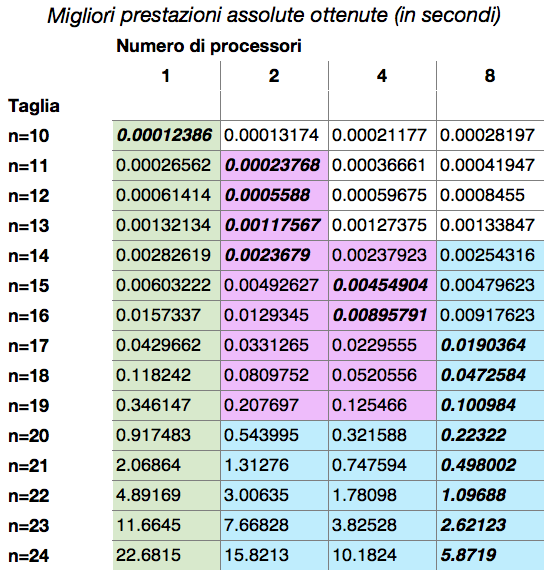
\includegraphics[width=0.65\textwidth]{immagini/best_performance}
  \caption{\small Tabella con i migliori tempi ottenuti con l'implementazione ottimizzata al variare di taglia,processori e \emph{blocking}. In verde i risultati sequenziali. In viola quelli con \emph{blocking \= unlimited}. In azzurro \emph{blocking \= unlimited}. In bianco nessun miglioramento. In grassetto il miglior tempo a parità di taglia}
\end{figure}

\begin{figure}[htp] 
  \centering
      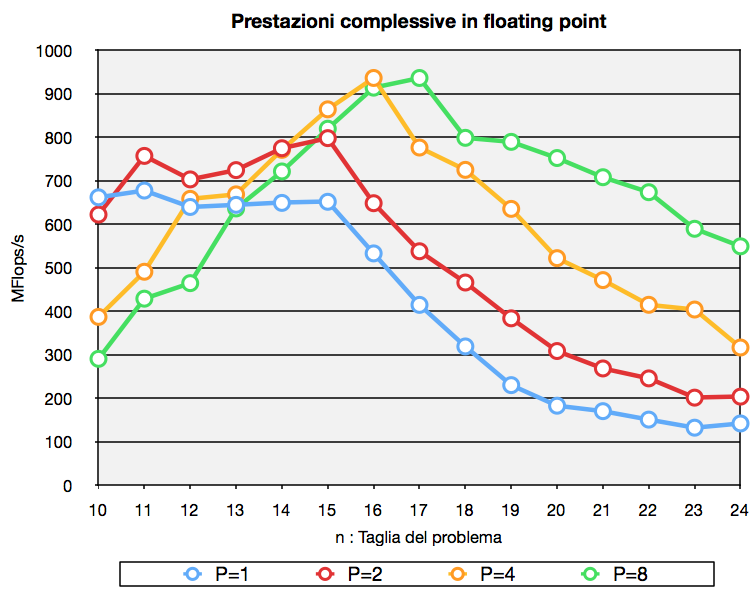
\includegraphics[width=0.70\textwidth]{immagini/mflips}
  \caption{\small MFlips/s al variare di taglia e \#processori}
\end{figure}
\end{document}